\section{代数方程式の解法}

\begin{frame}[t,fragile]{代数方程式}
  \begin{itemize}
    \setlength{\itemsep}{1em}
  \item 実係数の$n$次方程式
    \[
    P(z) = z^n + a_1 z^{n-1} + \cdots + a_n = 0
    \]
  \item ニュートン法 + 減次 (次数低下法)
    \begin{itemize}
    \item ニュートン法により一つの解($\alpha$)を求める
    \item $g(x) = f(x) / (x-\alpha)$の解として、他の解を逐次求めていく
    \item 毎回誤差がたまっていくため、解はくずれていく
    \end{itemize}
  \end{itemize}
\end{frame}


\begin{frame}[t,fragile]{Durand-Kerner-Aberth法 (Wierstrass法)}
  \begin{itemize}
    \setlength{\itemsep}{1em}
  \item 真の解を$\alpha_1,\alpha_2,\cdots,\alpha_n$とすると
    \[
    P(z) = (z-\alpha_1) (z-\alpha_2) \cdots (z-\alpha_n)
    \]
  \item $\alpha_1,\alpha_2,\cdots,\alpha_n$に現在の近似解$z^{(\nu)}_1,z^{(\nu)}_2,\cdots,z^{(\nu)}_n$を代入し、$z=z^{(\nu)}_k$における微分の値を評価
    \[
    P'(z^{(\nu)}_k) \approx \prod_{j \ne k} (z^{(\nu)}_k - z^{(\nu)}_j)
    \]
  \item ニュートン法による反復
    \[
    z^{(\nu+1)}_k = z^{(\nu)}_k - \frac{P(z^{(\nu)}_k)}{\prod_{j \ne k} (z^{(\nu)}_k - z^{(\nu)}_j)}
    \]
  \end{itemize}
\end{frame}

\begin{frame}[t,fragile]{初期値の選び方}
  \begin{itemize}
    \setlength{\itemsep}{1em}
  \item ある十分に大きな実数$r_0$を用いて
    \[
    z^{(0)}_k = - \frac{a_1}{n} + r_0 \exp \Big[ i \Big( \frac{2(k-1)\pi}{n} + \frac{\pi}{2n} \Big) \Big]
    \]
    複素平面上の中心$-a_1/n$、半径$r_0$の円周上の等間隔の点
  \item DKA法の収束
    \begin{itemize}
    \item $r_0$が十分大きい時
      \[\hspace*{-4cm} z^{(1)}_k + \frac{a_1}{n} \approx (1-\frac{1}{n}) (z^{(0)}_k + \frac{a_1}{n})
      \]
    \item 解の近傍では二次収束
    \item 解は互いに反発
    \item 例: $z^5-10z^4+43z^3-104z^2+150z-100=0$ (山本2003)
    \end{itemize}
  \end{itemize}
  \vspace*{-3.7cm}\hspace*{7.5cm}
  \resizebox{.3\textwidth}{!}{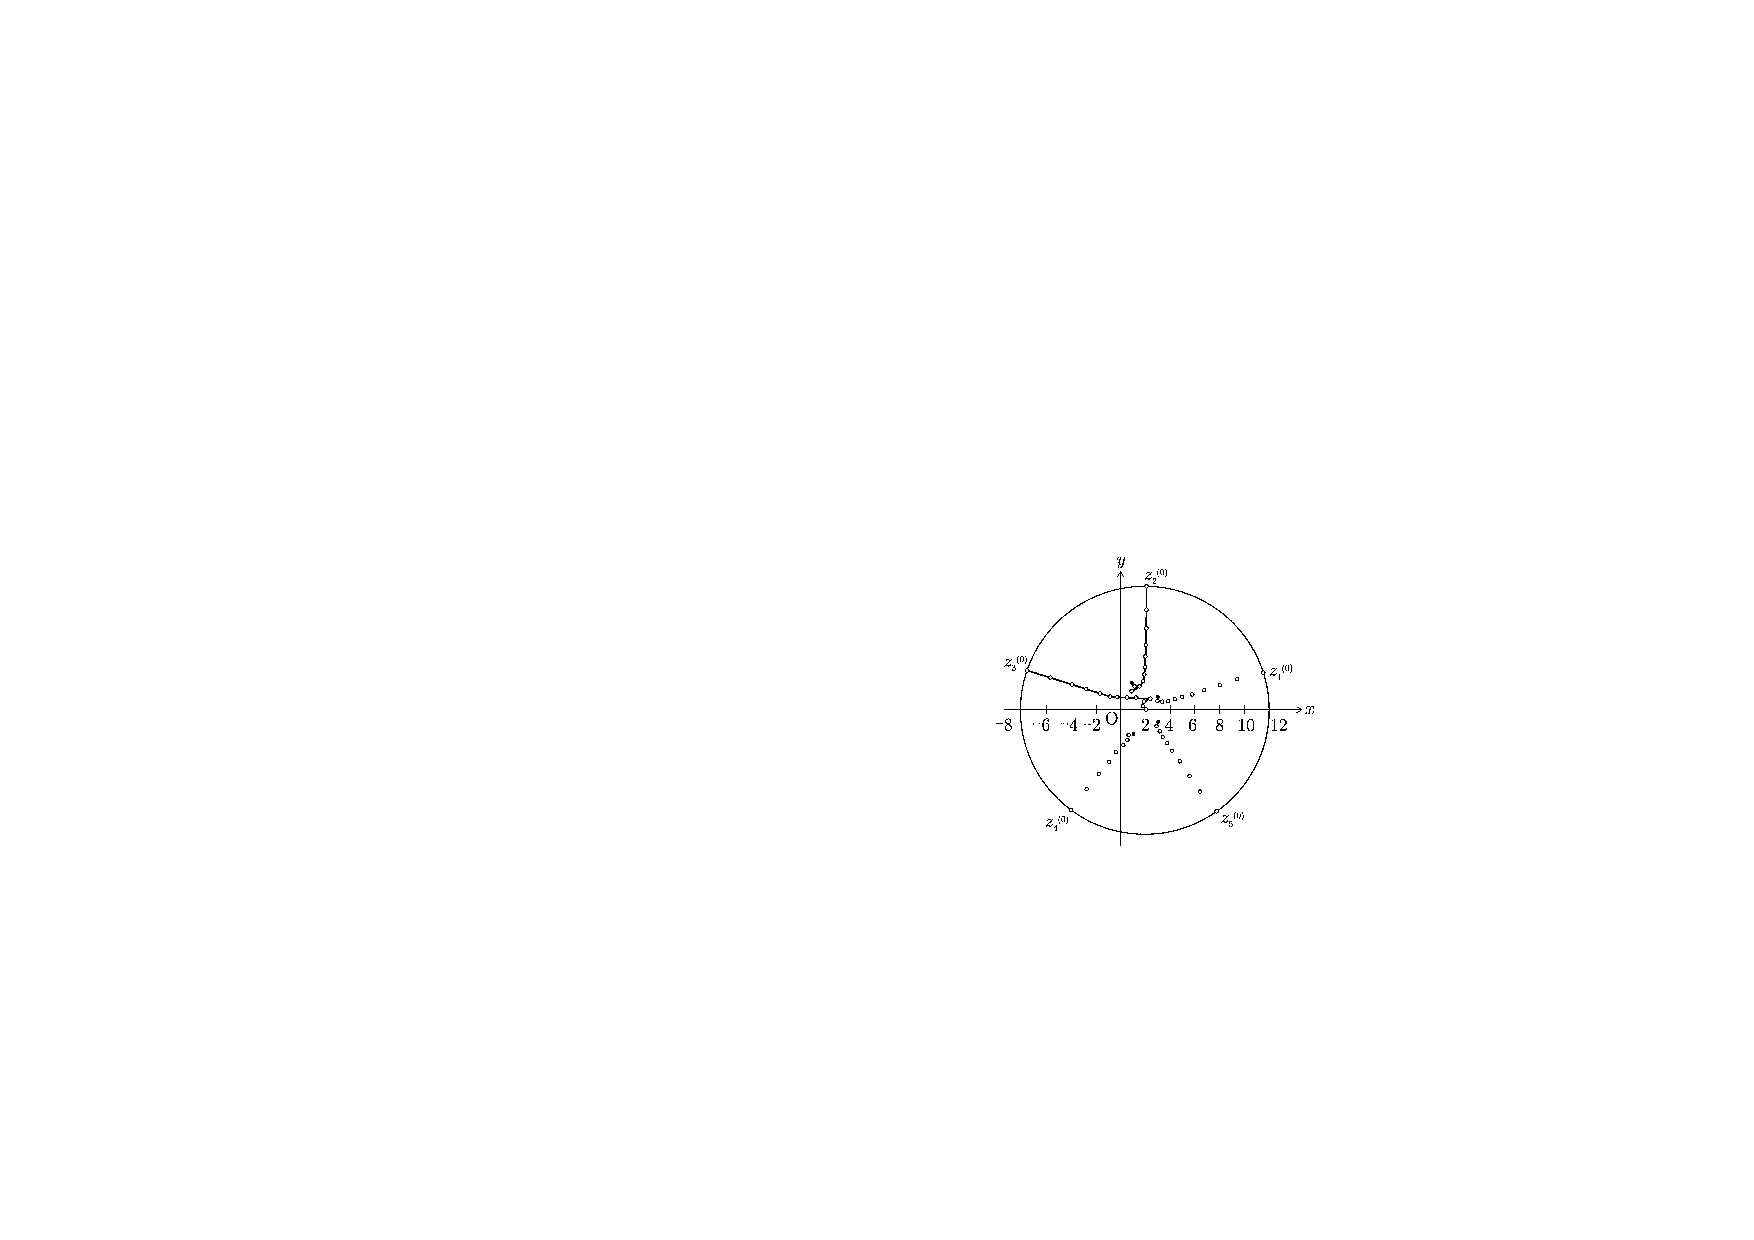
\includegraphics{image/DKA.pdf}}
\end{frame}
